\newpage
\section{Thiết kế hệ thống}
- Hệ thống sử dụng mô hình MVC(Model - Controller - View) để thiết kế.
\begin{itemize}
    \item View: \\
    - Customer View: Chế độ mặc định khi truy cập vào trang chính của hệ thống, không yêu cầu mật khẩu, chỉ yêu cầu khách nhập số bàn đang ngồi của mình (có dán tại bàn). Dành cho khách hàng xem món, đặt món, thanh toán, gọi phục vụ và gửi phản hồi.\\
    - Waiter View: Chế độ dành cho phục vụ Cho phép phục vụ nhận thông báo khi có khách gọi hoặc có món cần giao và nhấn nút Nhận để xác nhận đã có phục vụ tiếp nhận yêu cầu.\\
    - Kitchen View: Chế độ dành cho bếp. Cho phép bếp tiếp nhận món được đặt, xác nhận hoặc từ chối, chuyển trạng thái của món để hệ thống thông báo cho khách và phục vụ.\\
    - Manager View: Chế độ dành cho quản lý. Cho phép quản lý chỉnh sửa thông tin, thêm hoặc xóa món và đọc phản hồi của người dùng.
    \item Model:\\
    - Lấy thông tin các món ăn có trong danh sách món ăn\\
    - Thông tin giỏ hàng khi khách hàng đặt món\\
    - Danh sách đơn hàng\\
    - Xử lí các giao dịch khi thanh toán\\
    - Nhận thông tin khách hàng phản hồi
    \item Controller:\\
    - Hiển thị các món ăn và số bàn còn trống cho khách hàng\\
    - Thêm hoặc xóa món ăn của khách hàng trong giỏ hàng\\
    - Xử lý những tương tác của nhân viên và khách hàng.\\
    - Xử lý việc thanh toán và phản hồi của khách hàng.\\
    - Xử lý việc cập nhật menu và thông tin các món ăn của nhân viên.\\
    - Lưu lại giao dịch và đánh giá của khách hàng, chỉnh sửa menu (thông tin các món ăn, giá tiền.....).
\end{itemize}
\begin{figure}[!h]
    \begin{center}
        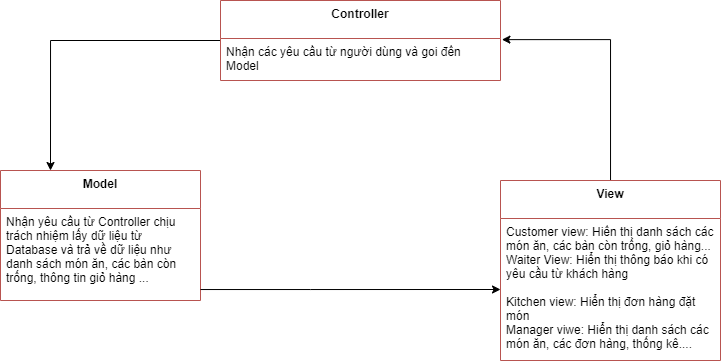
\includegraphics[scale=0.5]{Images/MVC.png}
    \end{center}
    \caption{Mô hình MVC}
\end{figure}
\newpage
\subsection{Deployment diagram}
\begin{figure}[!h]
    \begin{center}
        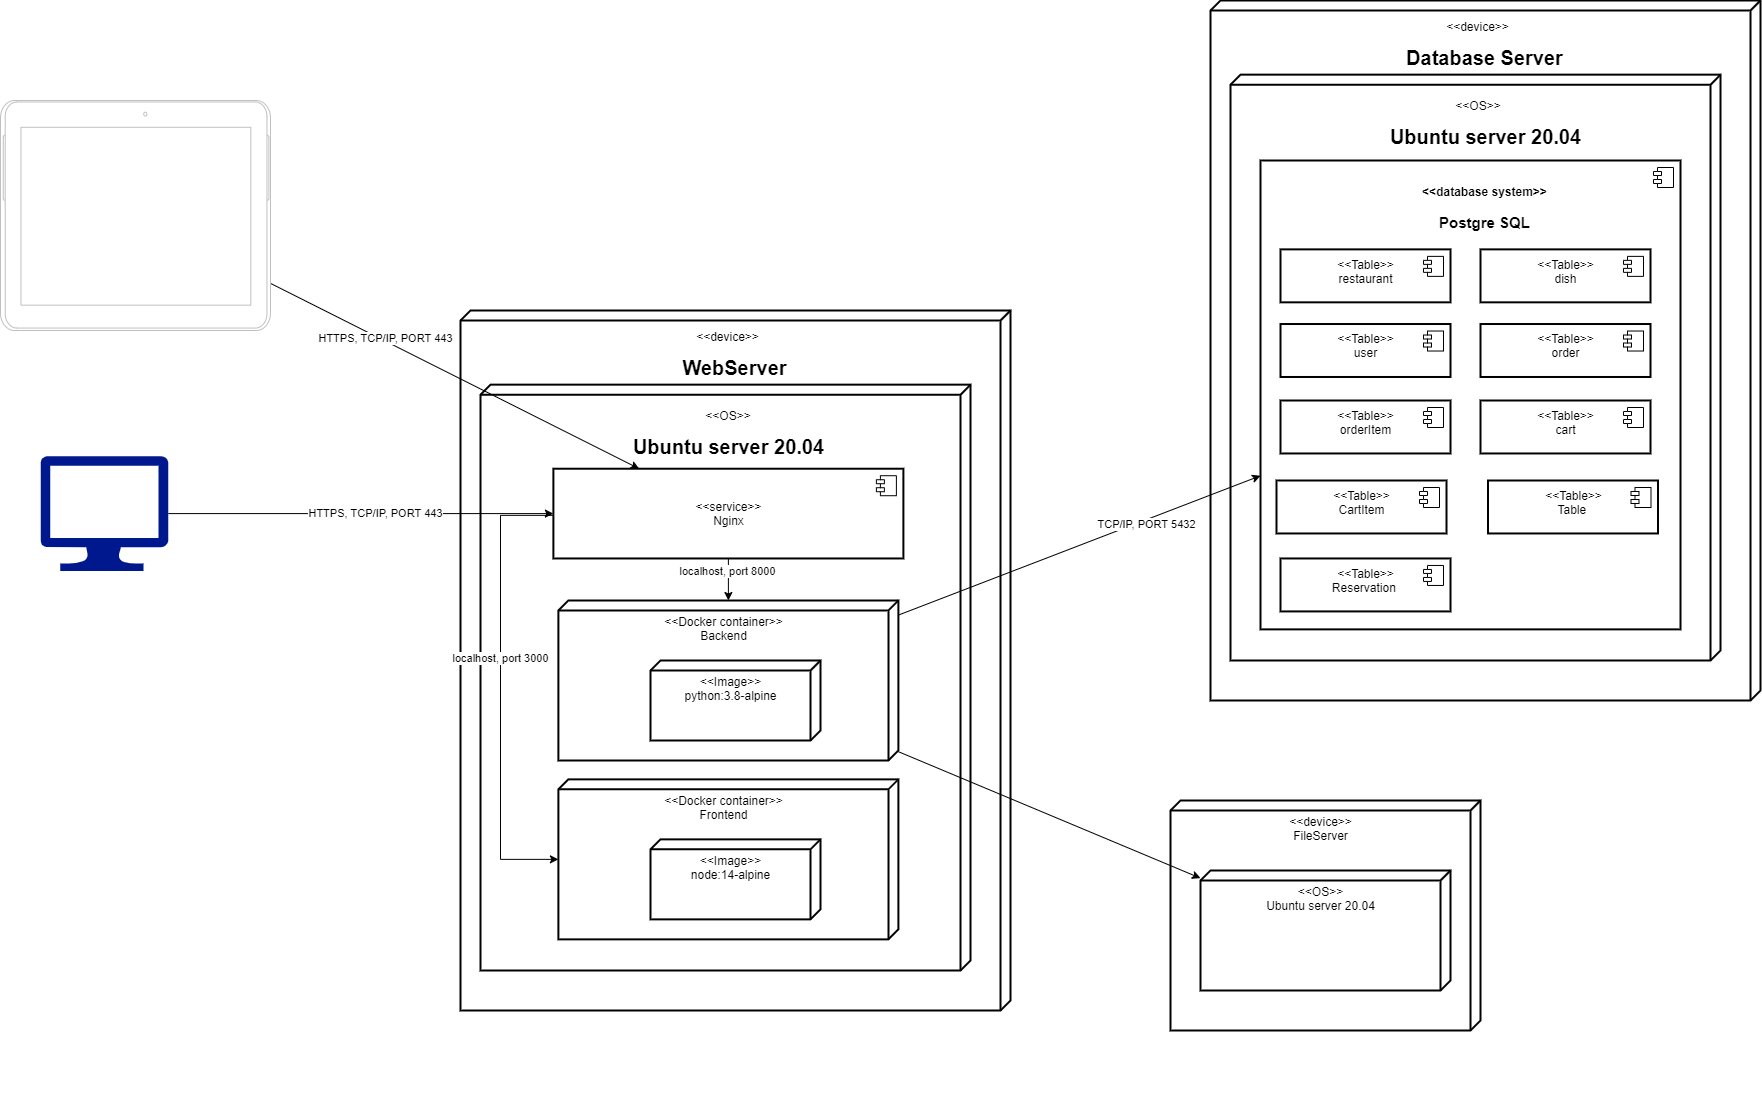
\includegraphics[scale=0.2]{Images/deploymet/SE_UML-deployment_diagram.png}
    \end{center}
    \caption{Deployment diagram}
\end{figure}
